\chapter{Grundlagen \& Stand der Technik}
%----------------------------------------------------------------------------------------
% Hier wird die Grundlage für das Verständnis der eigenen Lösung gelegt 
% Entweder nach der Einleitung oder am Schluss vor der Zusammenfassung der Arbeit 
% Stellen Sie hier dar wie andere sich dem Problem genähert haben was diese anderen Lösungen mit Ihrem Problem und Ihrer Lösung zu tun haben 
% Ordnen Sie Ihre eigene Lösung in den Gesamtkontext ein 
% wie unterscheidet sich Ihre Lösung 
% warum ist Ihre Lösung im Unterschied zu anderen gut 

Im Folgenden werden die Begriffe und Technologien definiert:

\section{Kernel}
Der Kernel ist ein Basisbestandteil des Betriebssystems. Dabei stellt der Kernel Basisfunktionen bereit, wie die Verwaltung der Hardware, von Prozessen, Nutzern oder Speicherzugriffen auf Cache, Arbeitsspeicher oder Laufwerken. In der folgenden Arbeit ist bei der Verwendung von Kernel der Linux Kernel gemeint. \cite[vgl.][S. 16 f.]{Baun.2017}

\section{Userspace \& Kernelspace}
\label{sec:user_kernelspace}
Der virtuelle Adressraum eines Prozesses wird in den Kernel- und Userspace unterteilt. Dabei ist der Kernelspace für den Kernel und der Userspace für den Prozess vorgesehen \cite[vgl.][101]{Baun.2017}. 
Wenn ein Prozess außerhalb des Kernels privilegierte Befehle, wie zum Beispiel das Schreiben einer Log Datei, ausführen soll, muss er dies dem Kernel mit einem Systemaufruf mitteilen.
Beim Systemaufruf erfolgt ein Sprung vom User- in den Kernelspace. Der Kernel übernimmt die Ausführung des Befehls und gibt die Kontrolle wieder an den Prozess zurück. \cite[vgl.][S. 135 f.]{Baun.2017}

Dieses Konzept ist tief in x86 Prozessoren verankert. Dabei wird jeder Prozess in einem von vier (0 bis 3) Ringen ausgeführt und kann diesen nicht selbständig verlassen. In Ring 0 läuft der Kernel und in Ring 3 die übrigen Prozesse. Bei einem Systemaufruf wird der Prozess in Ring 3 gestoppt und im Kernel in Ring 0 der Systemaufruf ausgeführt. Die Ringe 1 und 2 werden von modernen Betriebssystemen nicht genutzt.  \cite[vgl.][136, 235]{Baun.2017}

\section{Unikernel}
\label{sec:unikernel}
Ein Unikernel ist eine kleine, schnelle und sichere virtuelle Maschine ohne Betriebssystem. Der Unikernel soll skalierbar sein wie ein Container, die Anwendungen jedoch besser isolieren. Dafür werden die Ressourcen eines Computersystems nur einer einzigen Anwendung zur Verfügung gestellt und alle anderen Kernelfunktionen, die nicht benötigt werden, entfernt. Dies führt zur Reduzierung der Bootzeiten und des Speicherverbrauchs. 
Als Hardwareabstraktionsschicht wird ein Hypervisor verwendet, damit für neue Hardware keine neuen Bibliotheken entwickelt werden müssen.
Die verbreiteten Unikernels sind aktuell MirageOS, HalVM, IncludeOS, OSv und Rumprun. \cite[vgl.][256]{Jaworski.2020}

\section{Virtualisierung}
\label{sec:virtualiserung}

Virtualisierung ist eine Technologie, bei der die Ressourcen eines Computers oder Servers durch eine Softwareschicht zusammengefasst und weitergegeben werden. Dies ermöglicht eine bessere Ausnutzung der Ressourcen des Computers oder Servers. Dadurch lassen sich verschiedene Betriebssysteme oder Anwendungen auf demselben Computersystem betreiben. Der Server mit der realen Hardware wird Host genannt, die darauf laufenden Systeme als Gäste oder \acp{VM} bezeichnet. Virtualisierung kann laut Baun in die Bereiche Partitionierung, Hardware-Emulation, vollständige Virtualisierung, Paravirtualisierung, Hardware-Virtualisierung und Betriebssystem-Virtualisierung unterteilt werden. \cite[vgl.][231]{Baun.2017}

Partitionierung wird derzeit nur bei Großrechnern verwendet und definiert Teilsysteme eines Gesamtsystems. Jedes Teilsystem beinhaltet ein Betriebssystem und verhält sich wie ein eigenständiger Computer. Hardware-Emulation bildet innerhalb von Software die Hardware eines anderen Rechnersystems ab. Ziel ist, ein unverändertes Betriebssystem für eine andere Hardwarearchitektur auszuführen. Damit lässt sich zum Beispiel ein Programm für ARM auf einem x86 Computer ausführen. QEMU ist ein Beispiel für ein Hardware-Emulations Projekt. \cite[vgl.][233]{Baun.2017}

Mit vollständiger Virtualisierung ist es möglich, einer \ac{VM} ein vollständiges virtuelles System bereitzustellen. Dabei können Systemkomponenten emuliert werden. Die Zuteilung der Hardware übernimmt ein \ac{VMM}. Der \ac{VMM} läuft dabei in Ring 3, vgl. \ref{sec:user_kernelspace}, und der Kernel der \ac{VM} im ungenutzten Ring 1. Ein Systemaufruf vom Gastkernel wird dann vom \ac{VMM} verarbeitet und an den Hostkernel weitergegeben. Die Abbildung \ref{fig:virtualiserung} verdeutlicht diesen Aufbau. Beispiel für Lösungen, die auf dem \ac{VMM} aufbauen, sind Kernel-based Virtual Machine (KVM) und VMware. \cite[vgl.][S. 236 f.]{Baun.2017}

Bei der Paravirtualisierung wird ein Hypervisor verwendet, der direkt auf dem Computersystem installiert wird. Das Host Betriebssystem greift über den Hypervisor auf die Hardware zu und stellt die Gerätetreiber bereit. Der Hypervisor läuft dabei in Ring 0, das Host- und die Gastsysteme in Ring 1. Für den Hardwarezugriff stellt der Hypervisor Hypercalls zur Verfügung. Bei diesen wird der Systemaufruf aus den Gastsystemen verarbeitet und an den Kernel im Hostsystem weitergegeben. Diese Architektur ist in Abbildung \ref{fig:virtualiserung} dargestellt.  \cite[vgl.][S. 237 f.]{Baun.2017}

Mit aktuellen x86 Prozessoren lässt sich die Hardware-Virtualisierung verwenden. Hier wird die Privilegienstruktur um den Ring -1 erweitert. Dabei läuft der Hypervisor oder \ac{VMM} in Ring -1 und die \acp{VM} in Ring 0. Dadurch lassen sich alle Betriebssysteme ohne Anpassungen ausführen. Darüber hinaus hat das System in Ring -1 höhere Privilegien als die Systeme in Ring 0 und kann den Hardwarezugriff beeinflussen. Abbildung \ref{fig:virtualiserung} zeigt dieses Konzept. Die Betriebssystem-Virtualisierung wird auch Container-Virtualisierung genannt und wird in Abschnitt \ref{sec:container} beschrieben. \cite[vgl.][S. 237 f.]{Baun.2017}

\begin{figure}[hb]
	\centering
	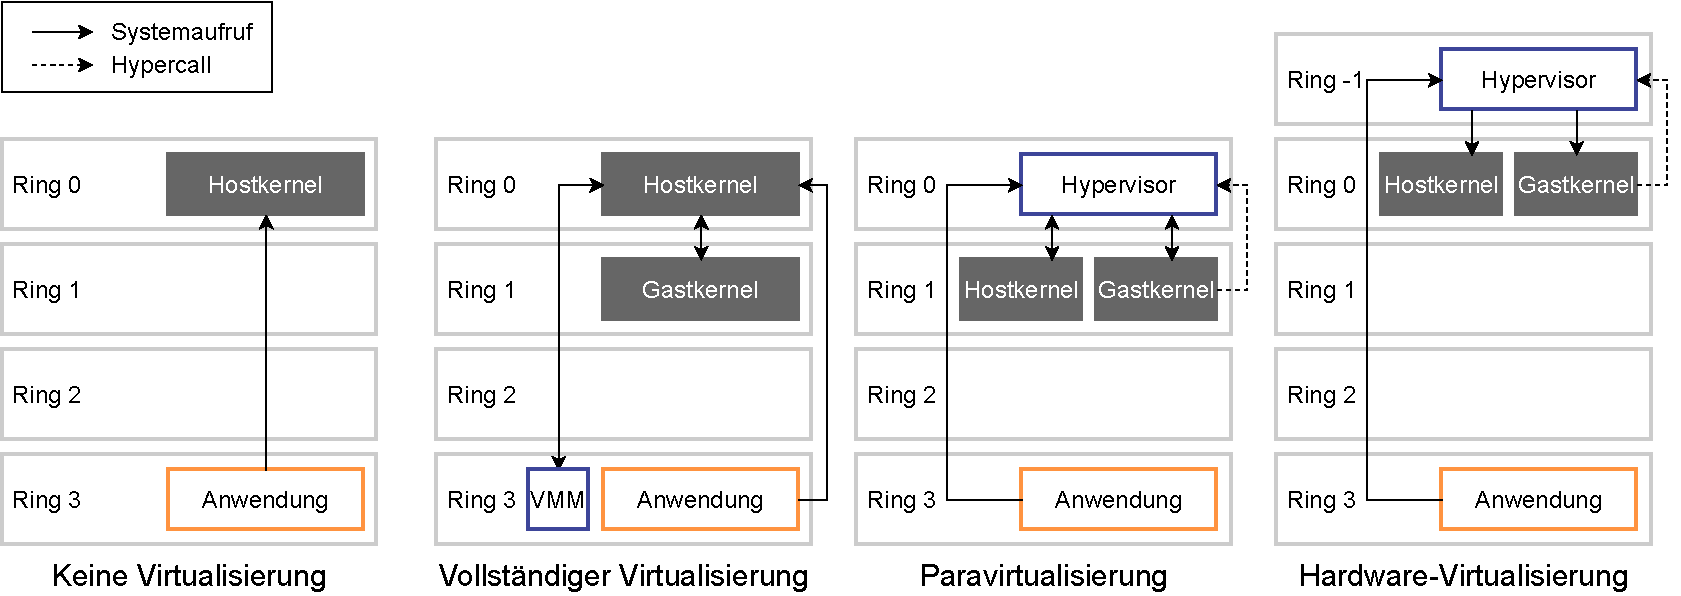
\includegraphics[width=1\linewidth]{gfx/virtualiserung.pdf}
	\caption{Virtualisierung im Vergleich}
	\footnotesize Quelle: In Anlehnung an \cite[vgl.][236, 238, 240]{Baun.2017}
	\label{fig:virtualiserung}
\end{figure} 

\section{Kernel-based Virtual Machine}
\label{sec:kvm}
\ac{KVM} ist eine Virtualisierungslösung mit der Architektur einer vollständigen Virtualisierung und unterstützt Hardware-Virtualisierung . \ac{KVM} ist seit 2007 Teil des Linuxkernels \cite[vgl.][8]{Peichert.20150928}. Neben \ac{KVM} existieren auch andere Produkte, wie beispielsweise VMware \cite[vgl.][237]{Baun.2017}. \ac{KVM} findet bei den in dieser Thesis betrachteten Technologien Verwendung und wird daher hier erläutert.
Bei \ac{KVM} lädt der Kernel beim Starten das benötigte Kernelmodul nach und ermöglicht den Betrieb von nahezu jedem Gastsystem. Wenn das Gastsystem mit \ac{QEMU} kompatibel ist, kann \ac{KVM} das Gastsystem mit sehr geringen Performanzverlusten ausführen. Wenn das System nicht kompatibel ist, emuliert \ac{QEMU} die Hardware. Diese Emulation ist deutlich langsamer \cite[vgl.][8]{Peichert.20150928}.

\section{Container}
\label{sec:container}
Container sind vergleichbar mit virtuellen Maschinen: Auch hier werden Anwendungen gekapselt auf einem System betrieben. Die Softwareschicht zwischen realem Computer und der Anwendung, die isoliert ausgeführt wird, ist gegenüber einer \ac{VM} deutlich reduziert. Beim Betrieb von Anwendungen in Containern sinken die Infrastrukturkosten gegenüber \acp{VM}, da viele Redundanzen wegfallen. Die Firma Docker nennt in einem Beispiel für Docker Container eine Reduktion um 66\% \cite[vgl.][]{BettyJunod.2017}.

Baun definiert Container-Virtualisierung im Artikel Servervirtualisierung folgendermaßen: "`Hier laufen unter ein und demselben Betriebssystemkern mehrere voneinander abgeschottete identische Systemumgebungen. Es wird kein zusätzliches Betriebssystem, sondern eine isolierte Laufzeitumgebung virtuell in einem geschlossenen Container erzeugt."' \cite[203]{Baun.2009}
Der Grafik \ref{fig:vmcontainer} sind die unterschiedlichen Schichten in den Architekturen von Containern und virtuellen Maschinen zu entnehmen.

Dabei werden die Kernel Funktionen Namespaces und Control Groups verwendet, um diese Applikationen voneinander zu isolieren \cite[vgl.][4]{Scholl.2019}.
Ein Container wird immer aus einem Containerabbild, dem Container Image, gestartet das einer Vorlage entspricht. Die Ausführung des Containers übernimmt dabei die Container Runtime. Damit ist, eine entsprechende Vorlage vorausgesetzt, eine Anwendung in einem Container in unter einer Minute betriebsbereit. Die Containerabbilder liegen in einem Standardformat vor. \cite[vgl.][S. 240 f.]{Baun.2017}
Dieses Format hat die \ac{OCI} in der "`Image Format Specification"' \cite[vgl.][]{OpenContainerInitiative.} festgelegt. Jede Software, welche die "`Runtime Specification"'  \cite[vgl.][]{OpenContainerInitiative.20200205} implementiert, ist dann in der Lage einen Container nach \ac{OCI} Spezifikation auszuführen \cite[vgl.][]{FerdinandThommes.20170720}.
Damit werden die Abhängigkeiten zur Ausführung eines Containers minimiert. Ein Container lässt sich, wie sein Vorbild in der Realität, einfach umziehen und fast überall starten \cite[vgl.][15]{Jangla.2018}. 

Die Unveränderlichkeit des Images hat verschiedene Auswirkungen: Bei der Inbetriebnahme eines Containers aus dem gleichen Image wird immer das gleiche Ergebnis entstehen. Damit ist es reproduzierbar. Auch werden alle Änderungen, die zur Laufzeit stattfinden, genau im Container gespeichert. Diese Änderungen lassen sich anzeigen, sodass sich ungeplante Änderungen oder Angriffe nachvollziehen lassen.
Ein Container speichert Daten nicht persistent, daher sind diese nach einem Containerneustart nicht mehr vorhanden. Mit Volumes können Daten im Container persistent gespeichert werden. Dazu wird ein Ordner auf dem Host-System an den Container weitergereicht und eingebunden.  \cite[vgl.][4]{Felter.2015}

\begin{figure}[hb]
	\centering
	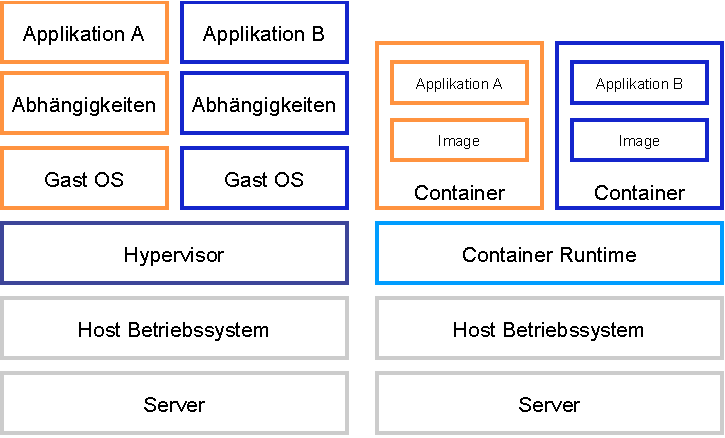
\includegraphics[width=1\linewidth]{gfx/vm_container.pdf}
	\caption{Virtuelle Maschine und Container im Vergleich}
	\label{fig:vmcontainer}
\end{figure}


\section{Docker}
\label{sec:docker}
Docker ist eine Entwicklerplattform für Container-Virtualisierung und wurde 2013 von der Docker Inc. veröffentlicht \cite[vgl.][10]{Jangla.2018}. Der Fokus von Docker liegt auf der Erstellung, Ausführung und Bereitstellung von Applikationen mithilfe von Containern \cite[vgl.][11]{Jangla.2018}.
Über den Docker Client wird die Docker Engine angesprochen. Durch diese Architektur kann ein Docker Client auf System A Container in der Docker Engine auf System B verwalten \cite[vgl.][55]{Poulton.2017}.
Die Docker Engine besteht dabei aus dem Docker daemon, containerd, Shim und der Runtime runc. Diese Bestandteile haben sich aus einem Docker daemon entwickelt. Die Trennung wurde vorgenommen, um die Entwicklung besser zu steuern und um Teile der Architektur tauschen zu können \cite[vgl.][55]{Poulton.2017}. 
Dabei stellt der Daemon die Schnittstellen bereit, um zwischen Docker Client und containerd zu kommunizieren. Die Kommunikation zwischen Client und Daemon erfolgt via REST API, die zwischen  Daemon und containerd via gRPC \cite[vgl.][60]{Poulton.2017}. 
Containerd ist für die Verwaltung der Container zuständig, dabei delegiert er an die Runtime. Containerd übergibt zum Beispiel das Image an runc \cite[vgl.][59]{Poulton.2017}. Containerd unterstützt dabei alle \ac{OCI} kompatiblen Runtimes und Images, vgl. \ref{sec:container}. Die Komponente Shim, englisch für Unterlegscheibe, fungiert als Entkopplung von Containerbetrieb und Administration. Dadurch lässt sich zum Beispiel eine Aktualisierung des Docker Daemons vornehmen, ohne dass der Betrieb der Container eingeschränkt wird  \cite[vgl.][S. 62 f.]{Poulton.2017}. Die Runtime runc ist für den eigentlichen Betrieb des Containers zuständig und leitet die Systemaufrufe aus dem Container an den Host Kernel weiter \cite[vgl.][59]{Poulton.2017}. Einen Überblick über die Architektur gibt die Abbildung \ref{fig:docker}.
Im weiteren Verlauf der Arbeit wird Docker häufig als Container Runtime bezeichnet, auch wenn die eigentliche Runtime runc ist. Dies dient der sprachlichen Vereinfachung und es ist in diesem Zusammenhang immer runc gemeint.

Docker nutzt verschiedene Linux-Funktionen, um die Container zu isolieren: Namespaces sorgen dafür, dass die Prozesse in einzelnen Containern, zueinander und zum Host System getrennt sind. Dadurch hat zum Beispiel jeder Netzwerk Namespace eine eigene IP-Adresse und ein eigenes Netzwerkinterface oder jeder Prozess seinen eigenen Prozessbaum. Docker verwendet Namespaces für die Isolierung von Prozessen, dem Netzwerk, Mounts, Inter-Prozess-Kommunikation, Nutzern und Hostnamen \cite[vgl.][S. 171 f.]{Poulton.2017}. In dem Buch "`Docker deep dive"' bezeichnet der Autor "`Container als organisierte Sammlung von Namespaces"'\footnote{Übersetzt aus: "`container is an organized collection of namespaces"' \cite[][172]{Poulton.2017}} \cite[][172]{Poulton.2017}.
Control Groups limitieren die Prozesse im Container. Damit ist eine Beschränkung der Nutzung von CPU, RAM und I/O möglich \cite[vgl.][172]{Poulton.2017}. Standardmäßig hat ein Docker Container keine Beschränkungen \cite[vgl.][]{DockerInc.2020}.
Mit Capabilities ist es möglich, einen Prozess in einem Container als nicht-root auszuführen, bestimmte Rechte, die eigentlich root voraussetzen, aber zu erlauben. Damit kann ein Container zum Beispiel bestimmte Netzwerkports verwenden \cite[vgl.][173]{Poulton.2017}.
Zusätzlich ist es möglich die Systemaufrufe durch runc mit Seccomp zu filtern. Im default Seccomp Profil sind 44 Systemaufrufe geblockt \cite[vgl.][]{DockerInc..20191203}. Seccomp, für "`secure computing"', ist eine Funktion des Linux Kernels, die Prozesse davon abhält bestimmte Systemaufrufe zu verwenden. Es sind nur die Aufrufe erlaubt, die im Seccomp Profil aufgeführt sind \cite[][S. 12 f.]{Randal.28.04.2019}.

Zunächst lief Docker nur auf Unix Systemen, seit Ende 2016 ist es auch mit Windows kompatibel \cite[vgl.][11]{Jangla.2018}. Dabei lassen sich unter Linux nur Linux Container und auf Windows entweder Linux oder Windows Container ausführen. Ein Mischbetrieb unter Windows ist nicht möglich \cite[vgl.][]{cwilhit.2019}. Dabei wird beim Betrieb eines Linux Containers unter Windows eine virtuelle Maschine gestartet, um den Linux Kernel in der \ac{VM} für die Containerausführung zu verwenden \cite[vgl.][28]{Poulton.2017}.

\begin{figure} [ht]
	\centering
	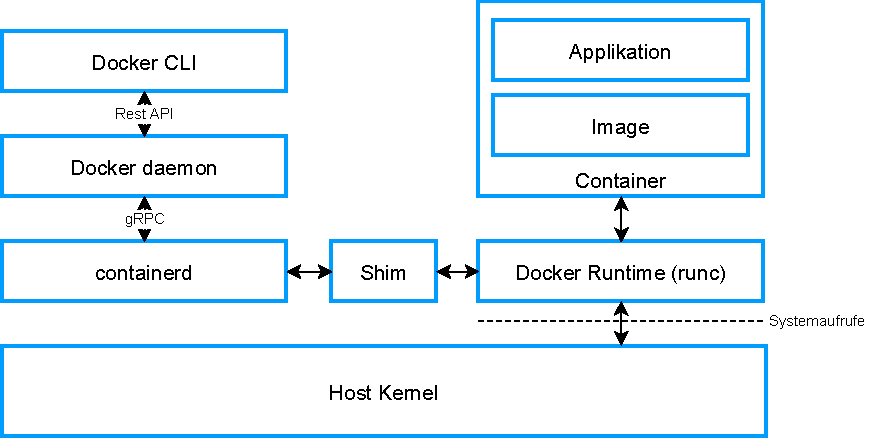
\includegraphics[width=1\linewidth]{gfx/docker_arch.pdf}
	\caption{Architektur von Docker}
	\label{fig:docker}
\end{figure}

\section{Docker Image}
Docker startet seine Container von Docker-Images aus. Ein Docker-Image ist eine Reihe von Datenschichten über einem Basis-Image. Die meisten Docker-Images starten von einem Basis-Image, wie zum Beispiel einem Ubuntu-Basis-Image \cite[vgl.][]{Ubuntu.20200220} oder Alpine-Basis-Image \cite[vgl.][]{Alpine.20200220}. 

Um mit mehreren Schichten eines Images eine einzige Dateisystemschicht zu bearbeiten, verwendet Docker ein spezielles Dateisystem namens Union File System. Dieses ermöglicht Dateien und Verzeichnisse in verschiedenen Dateisystemen zu einem einzigen konsistenten Dateisystem zusammenzufassen. \cite[vgl.][3]{Bui.13.01.2015}
Wenn Benutzer Änderungen an einem Container vornehmen, fügt Docker, anstatt die Änderungen direkt in das Abbild des Containers zu schreiben, eine zusätzliche Ebene hinzu, die diese Änderungen an dem Abbild enthält. Wenn der Benutzer beispielsweise MySQL in ein Ubuntu-Image installiert, erstellt Docker eine Datenschicht, die MySQL enthält und fügt dann dem Image eine weitere Schicht hinzu. Dieser Prozess macht den Image-Verteilungsprozess effizienter, da nur die aktualisierten Datenschichten verteilt werden müssen.

Die Docker Images werden in der Regel in einer Datenbank, einer Registry, vorgehalten, damit sie für die Ausführung eines Containers nicht neu erzeugt werden müssen \cite[vgl.][91]{Scholl.2019}. Dazu beherrschen die Container Runtimes häufig das Hoch- und Herunterladen von Container Images aus einer solchen Datenbank. Für diesen Prozess hat die Open Container Initiative einen Standard festgelegt, die "`Distribution Specification"' \cite[vgl.][]{HansJoachimBaader.20180410, OpenContainerInitiative.20200212}.

\section{Kubernetes}

Kubernetes ist eine Software, die zur Orchestrierung von Containern entwickelt und von Google 2014 veröffentlicht wurde  \cite[vgl.][7]{Scholl.2019}. Dabei bildet Kubernetes ein verteiltes System über alle Hosts des Kubernetes Clusters. Dadurch können Container, je nach Rechenlast, zwischen den einzelnen Host umverteilt werden, die Container skaliert oder die Kommunikation zwischen Containern auf verschiedenen Hosts sichergestellt werden \cite[vgl.][4]{Bernstein.2014}.
Derzeit ist Kubernetes die verbreitetste Orchestrierungslösung für Container \cite[vgl.][6]{sysdig.2019}.
Kubernetes unterstützt alle \ac{OCI} kompatiblen Runtimes für den Container Betrieb 
\cite[vgl.][7]{Scholl.2019}.

\section{Stand der Technik}
Ein Ansatz für die Absicherung von Container-Virtualisierung ist die Erhöhung der Isolierung. Dies kann durch verschiedene Herangehensweisen erreicht werden. Eine Möglichkeit ist Container in virtuellen Maschinen zu betreiben, eine andere die Container mit einem Kernel im Userspace zu verwenden. Weiter ist es möglich, Container in Unikernels einzusetzen. Für jede dieser Methoden wird in im Folgenden eine Lösung vorgestellt.
Die Grafik \ref{fig:zeitstrahl_vm_container} gibt einen Überblick über die Entstehung von vielen in der vorliegenden Arbeit benannten Technologien. Die genannten Begriffe sind im Zeitstrahl für die bessere Übersicht markiert.

\begin{figure}[hb]
	\centering
	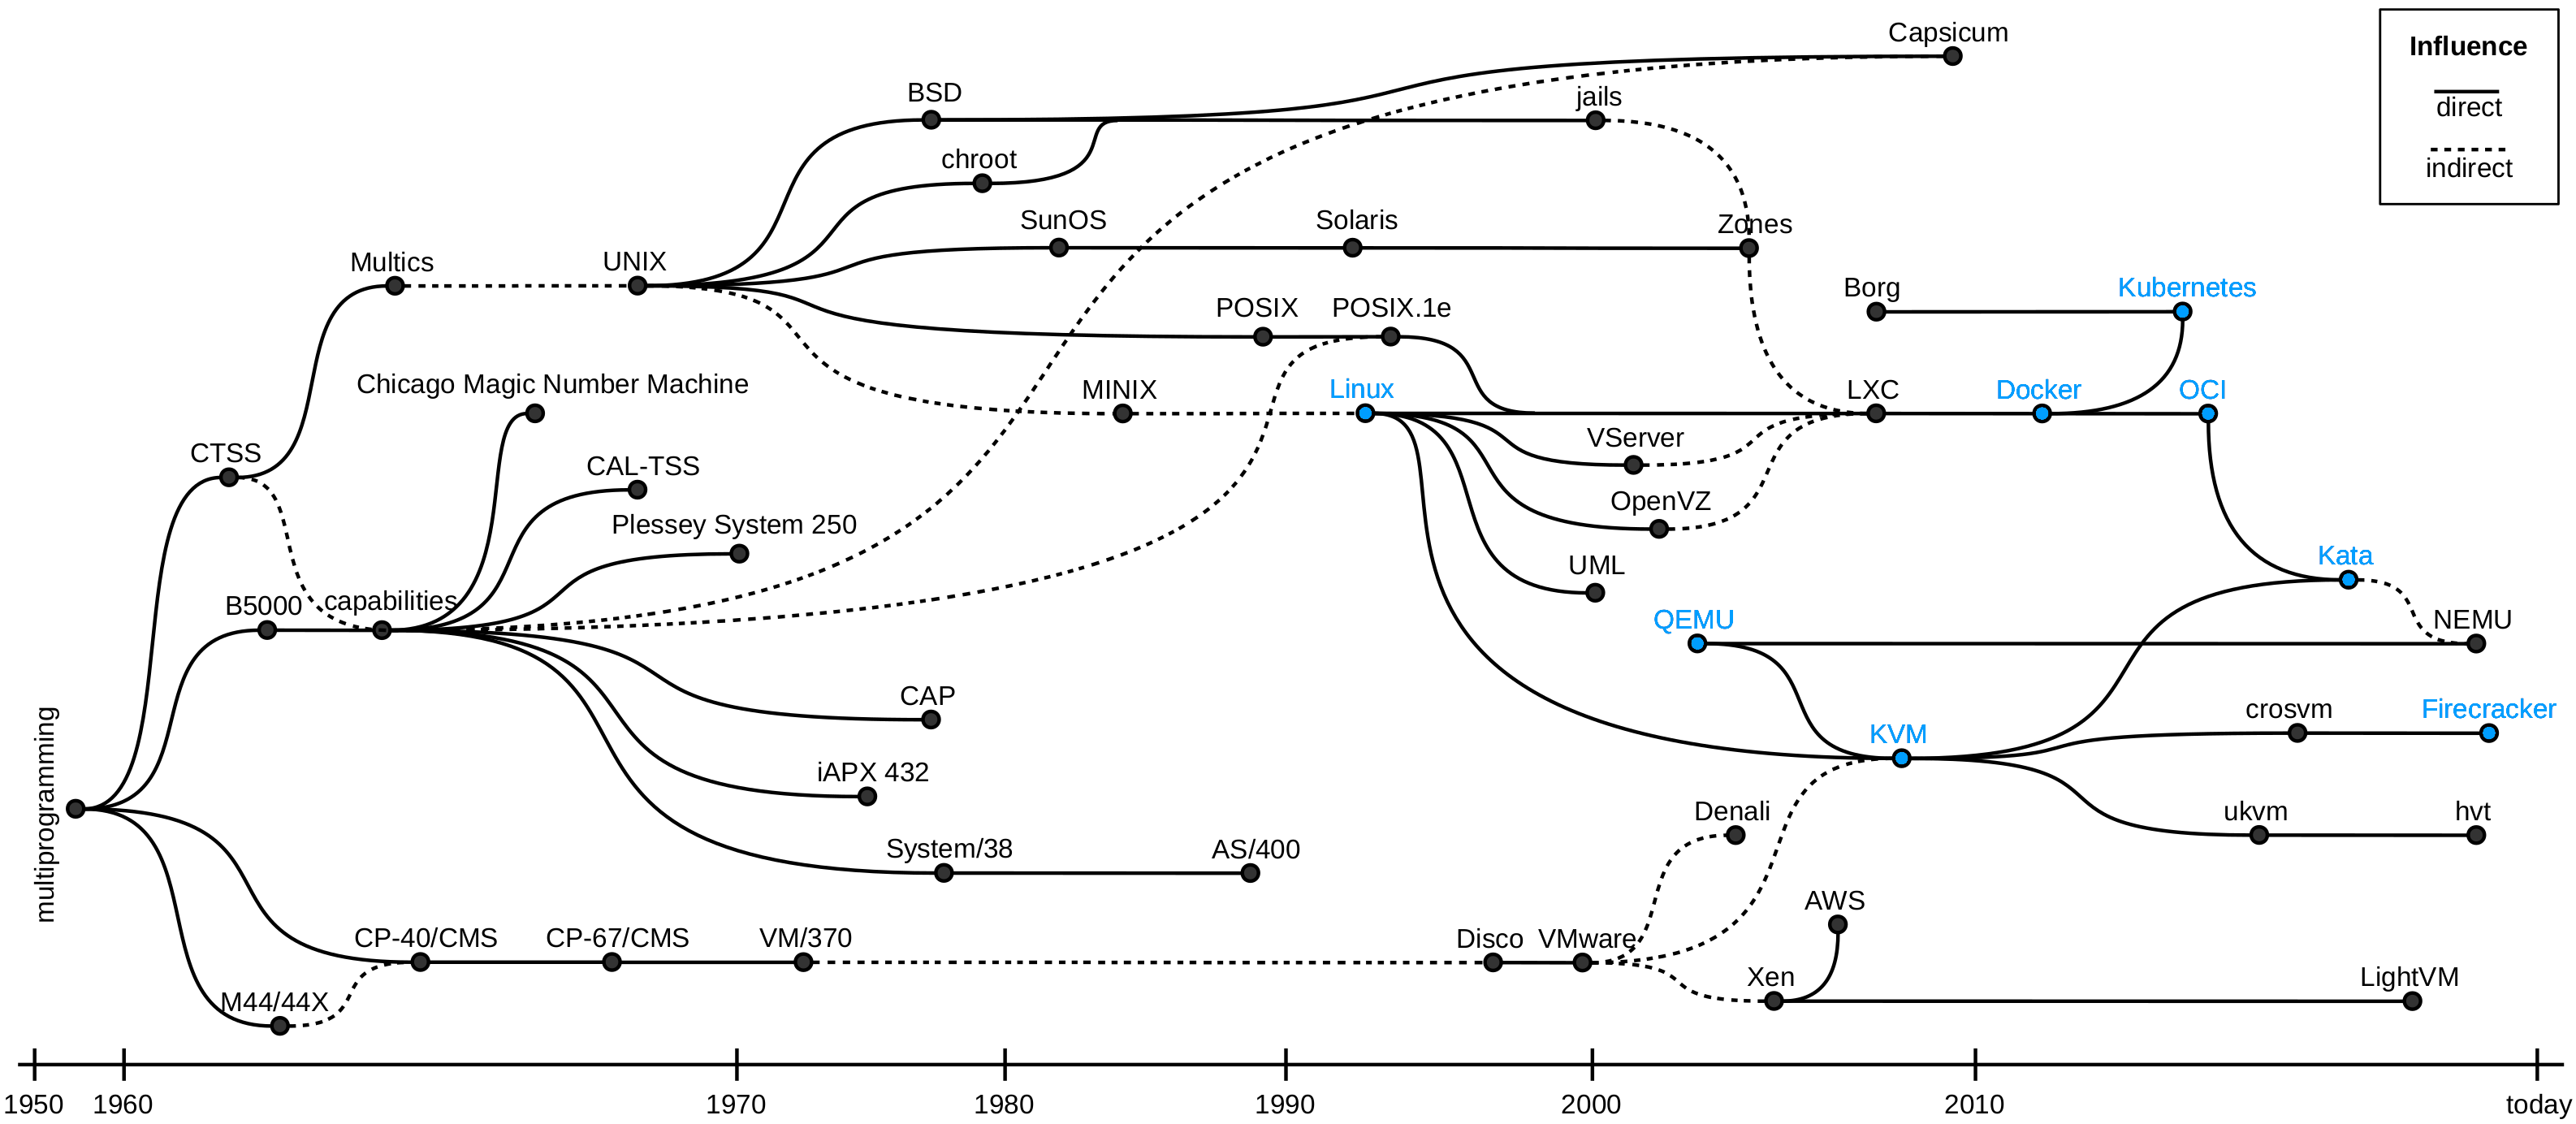
\includegraphics[width=1\linewidth]{gfx/VM_Container_Zeitstrahl.png}
	\caption{Die Entwicklung von Virtualisierung und Containern} 
	\footnotesize Quelle: In Anlehnung an \cite[][2]{Randal.28.04.2019}
	\label{fig:zeitstrahl_vm_container}
\end{figure}
\newpage

\subsection{Kata Containers}
\label{sec:kata}
Kata vereint die Isolierung von virtuellen Maschinen mit der unkomplizierten Nutzung von Containern \cite[vgl.][28]{TamHanna.01.11.2019}. Kata Container basiert auf den Technologien Hyper.sh und Intel’s clear containers  \cite[vgl.][6]{Scholl.2019}. Im Mai 2018 wurden diese beiden Projekte zusammengeführt und als Kata Containers veröffentlicht. Betreut wird das Projekt von der Open-Stack Foundation \cite[vgl.][106]{UdoSeidel.2018}.

Die Grundlage für die Virtualisierung bildet \ac{QEMU}, das auch in der Virtualisierung \ac{KVM} verwendet wird, vgl. \ref{sec:kvm}. Für jeden einzelnen Container startet Kata eine \ac{VM} \cite[vgl.][107]{UdoSeidel.2018}. Als Betriebssystem der virtuellen Maschine kommt Clear Linux zum Einsatz. Dieses Linux wurde von Intel auf Container optimiert und zielt auf einen möglichst geringen Ressourcenverbrauch ab  \cite[vgl.][107]{UdoSeidel.2018}. Da Kata \ac{QEMU} verwendet wird ein System mit Hardware-Virtualisierung vorausgesetzt  \cite[vgl.][108]{UdoSeidel.2018}.
Kata Containers beinhaltet auch eine \ac{OCI} kompatible Runtime, die sich neben der Runtime von Docker verwenden lässt \cite[vgl.][107]{UdoSeidel.2018}. Dadurch dass Docker die Container Runtime Schnittstelle nach dem Standard der \ac{OCI} implementiert hat, war es den Kata Entwicklern möglich, Kata in Docker zu integrieren \cite[vgl.][28]{TamHanna.01.11.2019}.
 
Damit eine Verwaltung des Containers in der \ac{VM} vom Host aus möglich ist, muss der Container für die Runtime, in diesem Fall kata-runtime, transparent sein. Dafür stellt Kata einen Shim bereit. Die Hauptaufgabe des Shims ist es, die I/O Verbindungen des Containers zu verwalten \cite[vgl.][]{katacontainers.20191207}. Dies wird mit den weiteren Elementen Proxy und Agent erreicht. Sie kommunizieren über die serielle Schnittstelle von \ac{QEMU} miteinander. Der Agent ist ein Prozess innerhalb der \ac{VM}. Pro \ac{VM} wird als Gegenstück auf dem Host ein Proxy gestartet. Die Abbildung \ref{fig:kata} verdeutlicht diese Architektur \cite[vgl.][107]{UdoSeidel.2018}.

Neben der Integration in Docker ist Kata Containers auch mit Kubernetes kompatibel. Es ist möglich, Kata und Docker parallel in einem Kubernetes Cluster zu betreiben und je nach Anwendung eine der Runtimes zu verwenden  \cite[vgl.][]{katacontainers.20191207}.
Die Entwickler stellen für viele Linux Distributionen Pakete zu Verfügung, mit denen sich Kata installieren lässt \cite[vgl.][]{katacontainers.20200120}. Weiter ist es auch möglich, Kata selbst zu kompilieren \cite[vgl.][108]{UdoSeidel.2018}.

\subsection{Kata Containers - Firecracker}
\label{sec:katafc}
Firecracker ist ein virtueller Maschinenmonitor, vgl. \ref{sec:virtualiserung}, der auf \ac{KVM} läuft, vgl. \ref{sec:kvm}. 
In der \ac{VM} wird ein minimaler Firecracker Kernel gebootet. Dieser hat eine sehr reduzierte Hardware Unterstützung. Für das Netzwerk Interface und den Zugriff von Daten sind bisher virtio net und virtio block implementiert \cite[vgl.][]{ArunGupta.2018}. Dadurch ist der Kernel besonders klein \cite[vgl.][11]{Randal.28.04.2019}. Für den Hersteller Amazon stand Geschwindigkeit, Sicherheit und Leichtgewichtigkeit im Fokus der Entwicklung \cite[vgl.][]{ArunGupta.2018}.

Kata Containers veröffentlichte mit der Version 1.5 die Unterstützung von Firecracker als Hypervisor. Dabei wird Firecracker anstelle von \ac{QEMU} verwendet, dies soll die Komplexität und den Ressourcenverbrauch verringern \cite[vgl.][11]{Randal.28.04.2019}.
Kata mit Firecracker, kurz Kata FC, ist zu Docker und Kubernetes kompatibel. Einige Funktionen wie die Verwendung von Ressourcenlimits, die Unterstützung von Container Volumes und Speicher Typen neben Block Speichern, fehlen bisher \cite[vgl.][]{katacontainers.20190123}. 

\begin{figure}[ht]
	\centering
	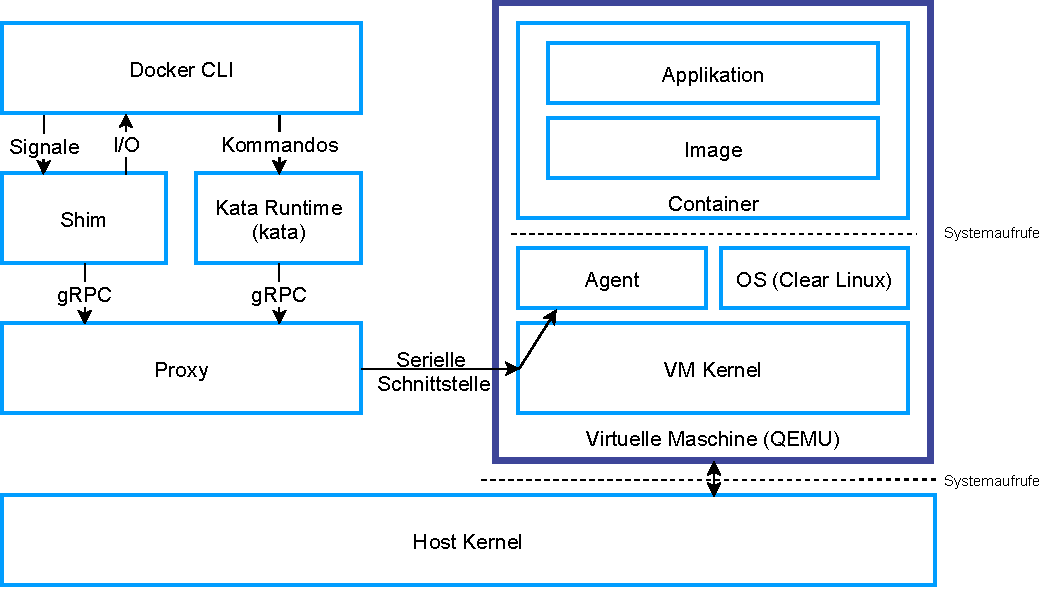
\includegraphics[width=1\linewidth]{gfx/kata_arch.pdf}
	\caption{Architektur von Kata Containers}
	\footnotesize Quelle: In Anlehnung an \cite[vgl.][ab 12:35]{NilsMagnus.20190425}
	\label{fig:kata}
\end{figure}

\subsection{gVisor}
\label{gvisor}
gVisor ist eine Container Runtime und ein an den Linux Kernel angelehnter Kernel im Userspace \cite[vgl.][6]{Scholl.2019}. 
Die Hauptbestandteile bilden Sentry und Gofer. Sentry beinhaltet den Kernel und läuft auf Linux. Gofer ist ein Proxy für die Dateiverarbeitung, der die Informationen dann an Sentry weiterleitet. Für die Kommunikation wird das Protokoll 9P verwendet \cite[vgl.][108]{UdoSeidel.2018}.
Die Abbildung \ref{fig:gvisor} veranschaulicht die Architektur von gVisor und verwendet die Datengrundlage aus der Arbeit "`The True Cost of Containing: A gVisor Case Study"' \cite[vgl.][]{EthanG.Young.2019}.

Sentry hat zwei Modi für die Verarbeitung von Systemaufrufen. Dabei werden im ptrace Modus Systemaufrufe unterbrochen und im \ac{KVM} Modus als Gast in einer \ac{VM} ausgeführt \cite[vgl.][2]{EthanG.Young.2019}.
Der Standardmodus ist ptrace, dies kann bei sehr rechenintensiven Aufgaben zu Performanzeinbußen führen. In solchen Fällen sollte die Verwendung von \ac{KVM} als gVisor Plattform zu einer Leistungssteigerung führen. Dies ist nur auf Systemen möglich, die Hardware-Virtualisierung unterstützen. \ac{KVM} als Plattform ist noch experimentell \cite[vgl.][109]{UdoSeidel.2018}.

Applikationen, die auf Sentry laufen, können laut Ethan Young 211 von den 319 Systemaufrufen unter Linux verwenden \cite[vgl.][2]{EthanG.Young.2019}. In der Systemaufrufkompatibilitätsreferenz von gVisor sind 166 Aufrufe als voll unterstützt markiert \cite[vgl.][]{gVisor.20200122}. Ein anderer Autor weist darauf hin, dass die implementierten Aufrufe dem Quellcode in der Datei "`gvisor/pkg/sentry/syscalls/linux/linux64.go"' zu entnehmen sind \cite[vgl.][108]{UdoSeidel.2018}.

Dabei nutzt Sentry für die Implementierung dieser Aufrufe selbst nur 55, die an den Host Kernel weitergegeben werden. Seccomp Filter verhindern, dass ein kompromittierter Sentry andere als diese 55 Systemaufrufe  verwendet.
Nach den gVisor Entwicklern werden die Aufrufe open und socket für die meisten Angriffe verwendet, um aus einem Container auszubrechen. Daher sind diese auch nicht unter den 55 erlaubten Aufrufen und die gVisor Bestandteile für den Netzwerk- und Speicherzugriff verzichten auf diese Systemaufrufe. \cite[vgl.][2]{EthanG.Young.2019}

\begin{figure}[hb]
	\centering
	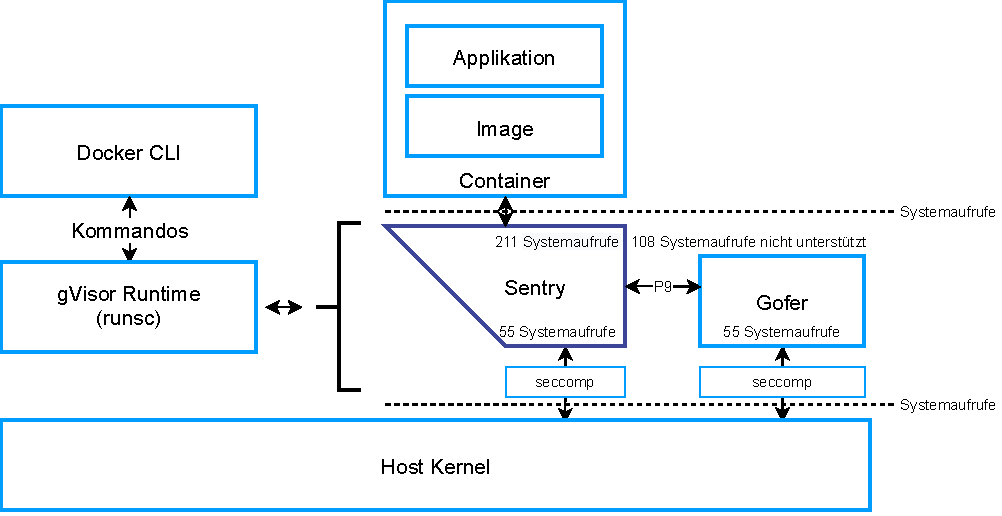
\includegraphics[width=0.9\linewidth]{gfx/gVisor_arch.pdf}
	\caption{Architektur von gVisor} 
	\footnotesize Quelle: In Anlehnung an \cite[][2]{EthanG.Young.2019}
	\label{fig:gvisor}
\end{figure}

Um die Angriffsvektoren in Bezug auf die Arbeit mit Dateien zu minimieren, wurden laut Young drei wichtige Muster implementiert: "`Erstens implementiert gVisor intern mehrere Dateisysteme [...]. Sentry kann in der Regel diese internen Dateisysteme verarbeiten, ohne den Host Kernel oder andere Helfer aufzurufen. Zweitens öffnen die Sentry-Dienste Aufrufe an externen Dateien [...] mithilfe von Gofer [...]; Gofer ist in der Lage, Dateien im Namen des Sentry zu öffnen und sie über einen 9P Kanal zurückzugeben. Drittens kann der Sentry, nachdem er ein Handle für eine externe Datei hat, Systemaufrufe aus der Anwendung lesen und schreiben, indem er ähnliche Systemaufrufe an den Host sendet.\footnote{Übersetzt aus: "`First, gVisor implements several file systems internally [...]; the Sentry can generally serve I/O to these internal file systems without calling out to the host or other helpers. Second, the Sentry services open calls to external files [...] with the help of [...] Gofer; the Gofer is able to open files on the Sentry’s behalf and pass them back via a 9P (Plan 9) channel. Third, after the Sentry has a handle to an external file, it can serve read and write system calls from the application by issuing similar system calls to the host."' \cite[][2]{EthanG.Young.2019}}"' \cite[][2]{EthanG.Young.2019}

Durch die eigene Implementierung des Kernels und den Verzicht auf einige Systemaufrufe ist gVisor nicht mit jeder Anwendung kompatibel. In der Dokumentation ist der jeweilige Implementationsstatus für jeden Systemaufruf ersichtlich \cite[vgl.][]{gVisor.20200122}. Eine Übersicht über getestet Anwendungen, die fehlerfrei laufen, ist der Dokumentation zu entnehmen \cite[vgl.][]{gVisor.20191025}.
Durch die Einhaltung der \ac{OCI} Standards ist die Runtime (runsc) von gVisor einfach mit Docker oder Kubernetes zu verwenden \cite[vgl.][108]{UdoSeidel.2018}.



\subsection{Nabla Containers}
\label{nabla}
Nabla Containers, kurz Nabla, erreicht eine hohe Isolierung durch die Filterung von Systemaufrufen vom Container Kernel zum Host Kernel \cite[vgl.][14]{Randal.28.04.2019}. Dabei basiert Nabla auf einem Unikernel, konkret wird Rumprun verwendet.
Ziel des Rumprun Projektes ist es, bestehende POSIX Anwendungen als Unikernel auf Hypervisoren auszuführen \cite[vgl.][256]{Jaworski.2020}.

Die Filterung wird durch seccomp in Kombination mit Solo5 vorgenommen. Erlaubt sind die folgenden sieben Systemaufrufe: read, write, ppoll, exit\_group, clock\_gettime, pwrite64 und pread6  \cite[vgl.][109]{UdoSeidel.2018}. Solo5 ist ein Portierung des Unikernels MirageOS auf \ac{KVM} \cite[vgl.][4]{Williams.2016}. Solo5 ist damit ein Bestandteil der Nabla Runtime und übernimmt die Systemaufruffilterung. Zusätzlich stellt es ein Interface bereit, auf dem Rumprun ausgeführt wird. Die Abbildung \ref{fig:nabla} veranschaulicht diese Architektur  \cite[vgl.][]{Nablacontainers.20190501}. 

Nabla verwendet zwei verschiedene Unikernels, um die Anwendung auszuführen und auf dem Host zu betreiben.
Eine Anwendung, die in einem Nabla Container ausgeführt werden soll, wird mit dem Rumprun Kernel zu einem ausführbaren Binary vereint. Dabei ist in einem solchen System nur eine Datei ausführbar. Dies ist nur möglich, wenn die Anwendung auf Rumprun lauffähig ist. Diese Einheit wird dann auf Solo5 ausgeführt \cite[vgl.][S. 109 f.]{UdoSeidel.2018}. 

Nabla hat die Projekte Solo5 und Rumprun geforked und an ihre Bedürfnisse angepasst. Dadurch sind nicht alle portierten Anwendungen für den ursprünglichen Rumprun Kernel mit Nabla kompatibel  \cite[vgl.][S. 109]{UdoSeidel.2018}.
Die Nabla Runtime (runnc) ist \ac{OCI} kompatibel, kann also mit Docker verwendet werden. Images nach dem \ac{OCI} Standard lassen sich aber nicht verwenden \cite[vgl.][S. 5 f.]{Scholl.2019}. 
Derzeit werden Container Volumes, Ressoucen Limits oder das Schreiben von Dateien außerhalb von /tmp noch nicht unterstützt  \cite[vgl.][]{nablacontainers.20190402}.

\begin{figure}[hb]
	\centering
	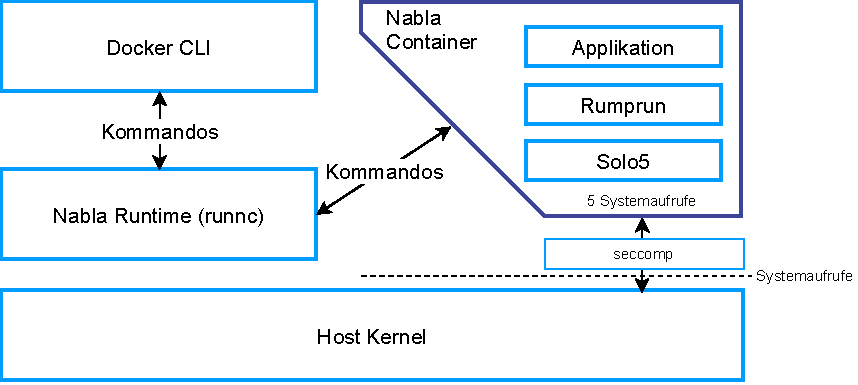
\includegraphics[width=1\linewidth]{gfx/nabla_arch.pdf}
	\caption{Architektur von Nabla}
	\label{fig:nabla}
\end{figure}

\section{Related Work}
\label{sec:relatedwork}

Der Autor Tam Hanna vergleicht Kata Containers mit Docker. Er bewertet Kata als sicherer, da es zur Ausführung ein virtuelles System verwendet. Weiter betrachtet er die Startzeit von Containern, die Antwortzeiten in einem Netzwerk und den Arbeitsspeicherverbrauch. In allen Disziplinen schneidet Kata schlechter ab als Docker. Die Messungen sind aber nur bedingt aussagekräftig, da diese kaum wiederholt werden und auch die unterschiedlichen Ressourcenlimits der Kandidaten nicht beachtet werden. \cite[vgl.][]{TamHanna.01.11.2019}

Im genannten Artikel wird die I/O Messung des Blogs stackhpc.com erwähnt. In diesem Beitrag wird die I/O Leistung auf einem Netzlaufwerk von einem echten Server, Docker und Kata betrachtet. Dabei ist Docker dem Server fast ebenbürtig, während Kata meist 15\% der Serverleistung erzielt. Die Latenz für das Schreiben oder Lesen von Dateien ist bei Docker und Kata signifikant schlechter, als die des Servers. \cite[vgl.][]{BharatKunwar.09.05.2019}

Die Kata Entwickler Xu Wang und Fupan Li vergleichen in einem Konferenzvortrag Kata und gVisor. Dabei verwendet der \ac{QEMU} Prozess in Kata weniger Systemaufrufe als gVisor. Der Verbrauch des Arbeitsspeichers ist bei Kata deutlich höher. Bei der Betrachtung der Startzeiten eines Containers liegt gVisor klar vor Kata und ist auch schneller als Docker. Der Vergleich der CPU Leistung zwischen Host, Kata und gVisor zeigt nur geringe Unterschiede. Der Overhead beim Schreiben in den Arbeitsspeicher ist bei Kata zwischen 2,5\% und 8\% und bei gVisor zwischen 5,5\% und 13\%. Die Ergebnisse im I/O Vergleich decken sich mit denen von \cite{BharatKunwar.09.05.2019}, wobei Kata mit aktiviertem "`passthru fs"' deutlich bessere Ergebnisse erzielt. gVisor ist beim Schreiben von 128 KB großen Dateien schneller als Kata, bei Dateien von 4 KB gleichauf. Zusammenfassend startet gVisor schneller und hat einen geringeren RAM Verbrauch. In fast allen anderen Disziplinen ist Kata schneller. \cite[vgl.][]{XuWang.2018}

In der Arbeit "`The True Cost of Containing: A gVisor Case Study"' wird gVisor mit Docker verglichen. gVisor ist sicherer als Docker, da bei einer Kompromittierung nur Sentry, ein Prozess im Userspace, und nicht der Host Kernel betroffen sei. Dabei ist gVisor deutlich langsamer. Im Detail ist Docker bei Systemaufrufen, Speicherzuweisungen und bei große Downloads mehr als doppelt so schnell und beim Öffnen von Dateien sogar über 200 mal schneller. \cite[vgl.][]{EthanG.Young.2019}

Der IBM Mitarbeiter James Bottomley vergleicht in einem Blog Beitrag Docker, Kata, gVisor und Nabla. Um die Leistung zu vergleichen, verwendet er die Antworten pro Sekunde von Redis, Python Tornado und Node Express. Docker erreicht den höchsten Durchsatz, gVisor den Niedrigsten. Kata und Nabla liegen dazwischen \cite[vgl.][]{JamesBottomley.14.07.2018}.
Zusätzlich führt er zu Bewertung der Sicherheit einer Container Runtime eine eigene Methode ein, das sogenannte "`Horizontal Attack Profile"'. Diese quantitative Methode misst die Codemenge im Linux Kernel, die vom laufenden System durchlaufen wird. Er nimmt an, dass die Fehlerdichte im Kernel gleich verteilt ist und je mehr Code ein Programm ausführt, desto mehr Programmierfehler sind potenziell ausnutzbar. Damit wäre ein Programm, das wenig Code im Kernel ausführt sicherer, als eines das viel Code ausführt. Dabei ist die Messung bei Containern mit dem Kernel Werkzeug ftrace unkomplizierter als bei Hypervisoren oder \ac{VMM}. Bei der Messung wird die Anzahl der aufgerufenen Funktionen, nicht die der durchlaufenen Codezeilen erhoben.
Nach dieser Methode ist Nabla deutlich sicherer als Docker. Kata und gVisor verwenden fast genauso viele Funktionen im Kernel wie Docker. \cite[vgl.][]{JamesBottomley.14.07.2018, Luksa.2018}

Die Entwickler von gVisor vergleichen in ihrer Dokumentation die Leistung von gVisor mit Docker. Bei Betrachtung der Arbeitsspeicherzugriffe und CPU gibt es wenige Unterschiede zwischen gVisor und Docker. Bei der Berechnung eines neuronalen Netzwerks mit TensorFlow ist Docker schneller. Die Laufzeit von Systemaufrufen ist bei gVisor deutlich länger als bei Docker, mit der Verwendung der \ac{KVM} Plattform in gVisor sinkt die Laufzeit deutlich unter den Wert von Docker. Die Startzeiten von Containern sind vergleichbar. Die Transferrate bei der Übertragung von Dateien ist bei Docker deutlich höher, als bei gVisor. Die Entwickler führen an, dass die Leistungsnachteile von gVisor bei gemischten Lasten in den Hintergrund treten und mit Docker vergleichbar sind. \cite[vgl.][]{gVisor.20200122b}

\section{Forschungsbedarf}

Da sich Prozesse mit Container-Virtualisierung unkomplizierter automatisieren lassen als mit virtuellen Maschinen, soll aus diesem Grund nach einer Verbesserung der Isolierung bei Container-Virtualisierung geforscht werden. Weiter hat die Container-Virtualisierung eine kürzere Historie als virtuelle Maschinen und haben daher eine modernere Architektur. Der Autor Allison Randal von "`The Ideal Versus the Real: Revisiting the History of Virtual Machines  and Containers"' kommt zu dem Schluss, dass Container gegenüber virtuellen Maschinen im Fokus stehen sollten, wenn an der Erhöhung der Isolierung geforscht wird. Der Grund dafür sei nicht, dass die bisherige Umsetzung in Container Runtimes besser wäre, als in anderen Virtualisierungslösungen, sondern weil Container eine modulare Architektur besitzen. Das ermöglicht einen flexibleren Umgang mit unterschiedlicher Software und Hardware Architekturen.  \cite[vgl.][15]{Randal.28.04.2019}

Weiter gibt es wenige Vergleiche der Kandidaten Kata, gVisor und Nabla, vgl. \ref{sec:relatedwork}, was wahrscheinlich auf die vergleichsweise kurzen Erscheinungszeiträume zurückzuführen ist. Kata,  gVisor und Nabla wurden 2018 veröffentlicht \cite[vgl.][106]{UdoSeidel.2018, NicolasLacasse.2018052, VaughanNichols.20180716}. Es fehlt zudem eine allgemein anerkannte Methode für einen solchen Vergleich.
Die vorliegende Arbeit schießt diese Lücke und legt Kriterien dar, mit denen sich verschieden Runtimes vergleichen lassen. Um dies zu fördern, wird die Performanzmessung wiederverwendbar entwickelt und veröffentlicht\footnote{Das Projekt ist hier einzusehen: \href{https://github.com/timstoffel/container_runtime_benchmark}{github.com/timstoffel/container\_runtime\_benchmark}}.
Mit dieser Vorlage lassen sich verschiedene Container Runtimes gegenüberstellen.